\chapter{Fertigstellung}
Alle einzelnen Komponenten sind nun bereits fertiggestellt. Der Raspberry Pi sitzt sicher hinter
dem Touchscreen, welcher sicher auf der Box liegt. Der Rahmen und das Türblatt bilden die
Modelltür und die elektronische Schaltung ist ebenso voll funktionsfähig.

\section{Zusammenführung}

Das Schloss wurde mit Schrauben an den Türrahmen und das Türblatt befestigt.
Der nächste Schritt war es, mit kleinen Schrauben die Elektronik-beinhaltende Box
seitlich an den Türrahmen zu montieren.
Als letztes musst das elektronische Schloss an den GPIO-Pin des Raspberry Pis angeschlossen werden.

Das Vorzeigemodell war somit vollendet und voll funktionsfähig.

\section{Das Endprodukt}
\begin{figure}[H]
    \begin{center}
        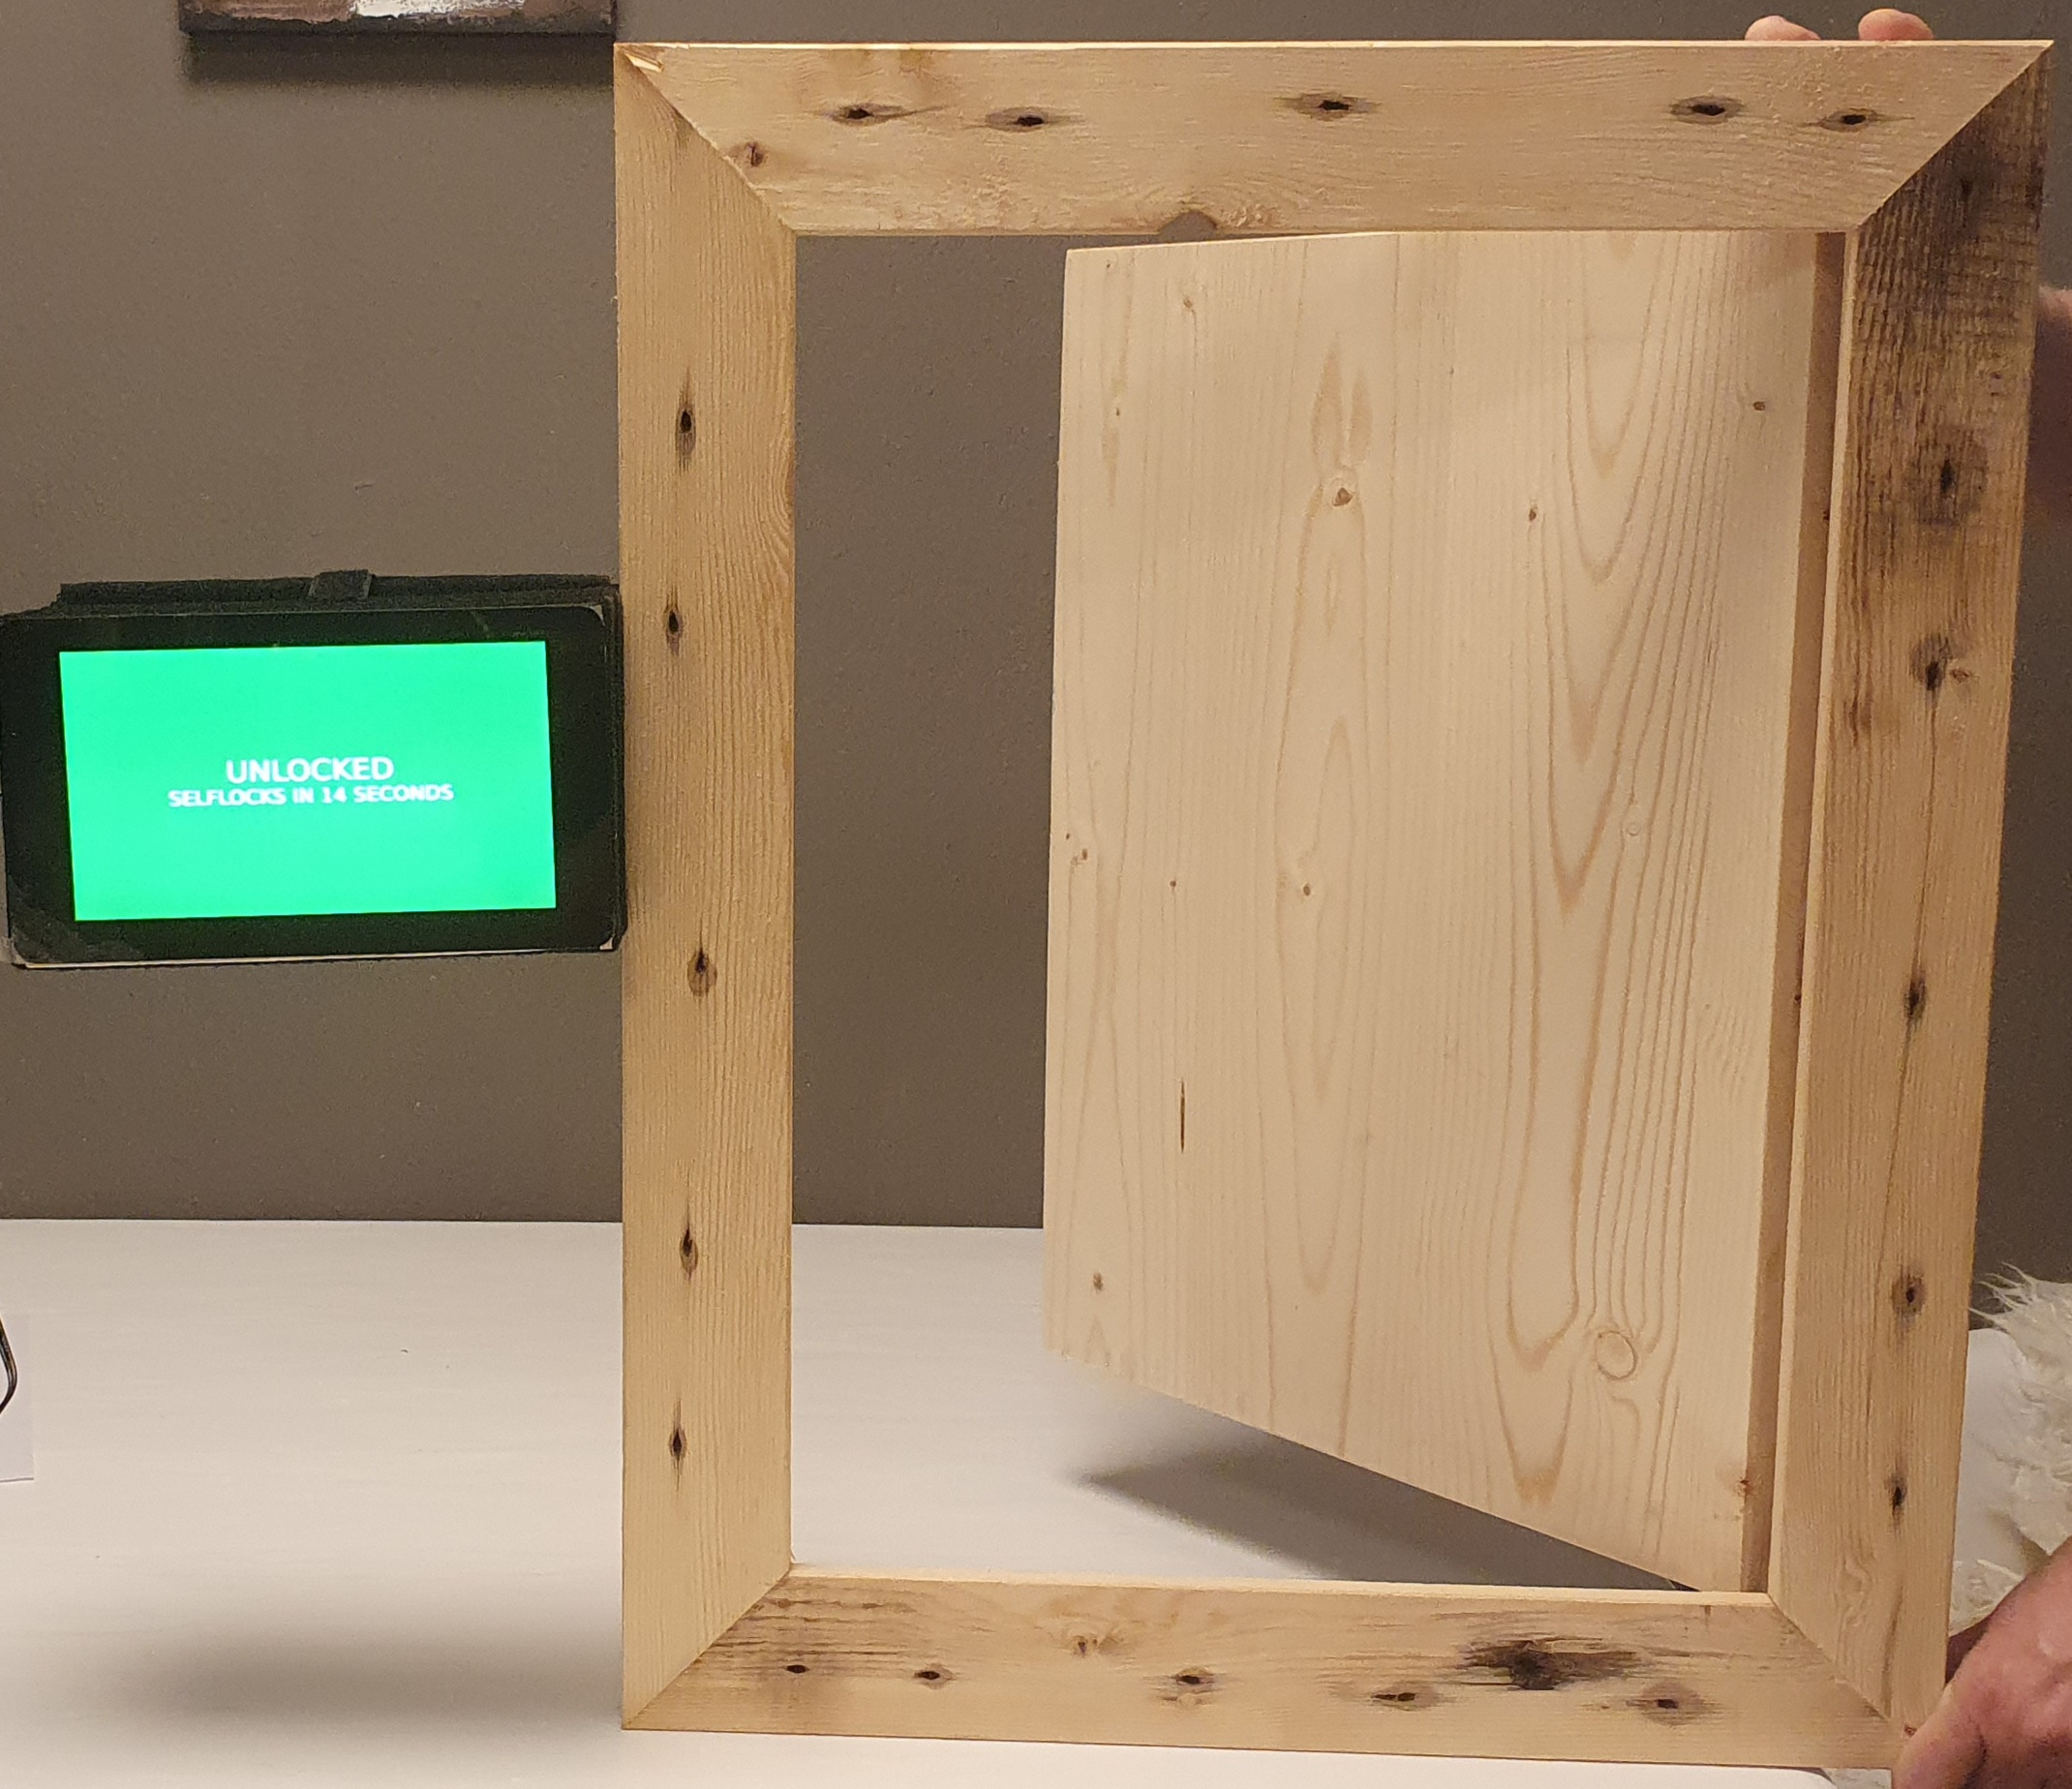
\includegraphics[width=0.9\textwidth]{images/core/fertig.jpg}
        \caption{Das Vorzeigemodell}
    \end{center}
\end{figure}